% IFAC International Federation of Automatic Control paper template. 
% Created by: ?
% Modified by: Rasmus Christensen, Aalborg University, Denmark 15/12/2012
\documentclass{ifacconf}

\usepackage{natbib}            % you should have natbib.sty
\usepackage{graphicx}          % Include this line if your 
                               % document contains figures,
%\usepackage[dvips]{epsfig}    % or this line, depending on which
                               % you prefer.
\usepackage[utf8]{inputenc} % So we can input Nicks name in the paper title!
\usepackage[T1]{fontenc}
\usepackage{amsmath,amsfonts,amssymb} % Added so we can do pretty math equations.

% predefined environments
%\begin{thm} ... \end{thm}		% Theorem
%\begin{lem} ... \end{lem}		% Lemma
%\begin{claim} ... \end{claim}	% Claim
%\begin{conj} ... \end{conj}	% Conjecture
%\begin{cor} ... \end{cor}		% Corollary
%\begin{fact} ... \end{fact}	% Fact
%\begin{hypo} ... \end{hypo}	% Hypothesis
%\begin{prop} ... \end{prop}	% Proposition
%\begin{crit} ... \end{crit}	% Criterion


\begin{document}

\begin{frontmatter}

\title{Centralized State Estimation of Distributed Maritime Autonomous Surface Oceanographers\thanksref{footnoteinfo}} % Title, preferably not more than 10 words.

\thanks[footnoteinfo]{Thanks to the  has been paid for in full by the School of Information Communication and Technology.}

\author[First]{Rasmus L. Christensen} 
\author[First]{Frederik Juul} 
\author[First]{Nick \O stergaard}
\author[First]{Attila Fodor}
\author[First]{Tudor Muresan}
\address[First]{Department of Electronic Systems, Aalborg University, Fredrik Bajers Vej 7, 9220 Aalborg \O st, Denmark (e-mail: \{ralch,nickoe,fjuul,tudor,attila\}@es.aau.dk)}                                            
          
\begin{keyword}                           % Five to ten keywords,  
Path planning; Centralised control; Baud rates; State estimation; Marine systems; Master slave system;              % chosen from the IFAC 
\end{keyword}                             % keyword list or with the 
                                          % help of the Automatica 
                                          % keyword wizard


\begin{abstract}                          % Abstract of not more than 250 words.
This paper considers the subject of running a centralized controller for the purpose of navigating a small Autonomous Surface Vehicle (ASV). The centralized controller is using a Kalman filter as a state predictor to improve the precision of the navigational aids mounted aboard. The work presents the design of the motion control system as well as the development of a protocol used to push through as much data on a standard 9.6 kbps data link simplex link.

The performance for the algorithms developed in this project, have been tested in Limfjorden in Aalborg, and towards the end, results of these tests are shown. 
\end{abstract}

\end{frontmatter}

\section{Introduction}
As up to date mapping of the coastal areas around Greenland is not available, and the process of creating these are a both time consuming and expensive task. One way to reduce both the costs and the amount of time invested in such a project could be to develop small autonomous drones to carry out this task. 

These drones should be controlled by a mothership, which would utilize a simple data link, both to preserve bandwith, but also to make the duration at which the ships are able to sail as long as possible, by limiting the power consumption. 

Currently the main focus of autonomous vehicles have been on aerial, ground and underwater vehicles, why there is close to no research going on about small autonomous surface vessels. An example of such a vessel is the Stingray ASV developed by Isreali Based Elbit Systems. The purpose of this vehicle is somewhat military related, where the purpose of measuring the coastal areas around Greenland are purely humanitarian,

{\bf Do not change the font sizes or line spacing to squeeze more text into a limited number of pages. Use italics for emphasis; do not underline}.

\subsection{Problem statement}
\begin{hypo} Is it possible to develop a centralized state estimator for use in the maritime environment using a small data link \end{hypo}

\subsection{A subsection}

\begin{figure}
	\begin{center}
		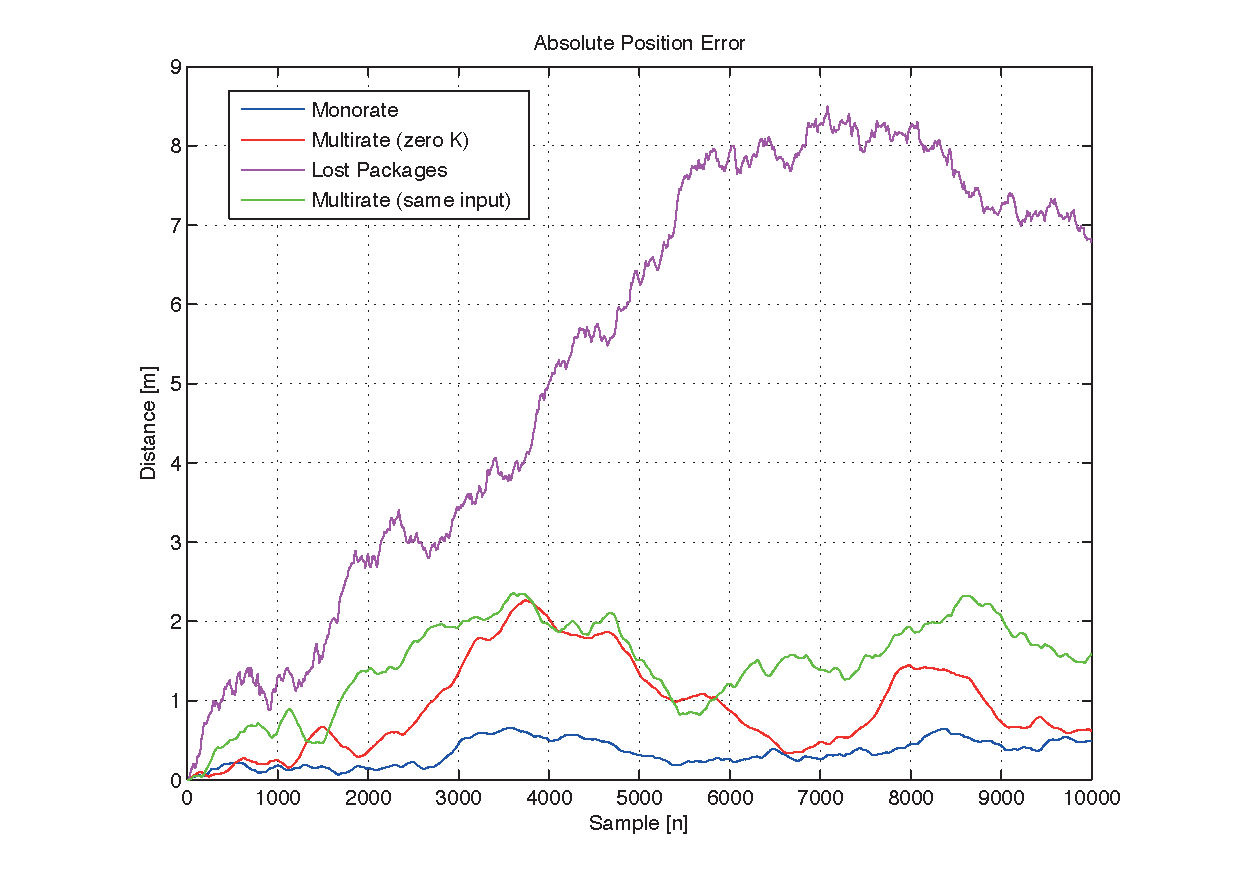
\includegraphics[width=8.4cm]{img/10percent} % width of a column is 8.4 cm.
		\caption{Bifurcation: Plot of local maxima of $x$ with damping $a$ decreasing}  
		\label{fig:fig1}
	\end{center}
\end{figure}

\section{Methods}

The methods developed in this project - and the papers. 2

\subsection{Path planning algorithm}

The path planning algorithm is based around the train-track transition problem originally solved in \citep{Art:1}, which divides the path into straight and turning parts and describes the transition between these using the normalized Fresnel integral, describing an Euler spiral, which allows the ship to maintain a linear acceleration through the turn, thus keeping the amount of jerk $j$ as close to zero as possible. A series of key points are generated in the turn, which determine a path that meets the above requirements \citep{Art:2}. The two Fresnel integrals are given as in equation (\ref{eq:fresnel}):
\begin{align}
C_F(x) = \int_0^x \cos(t^2)dt,\,\,\,\,S_F(x) = \int_0^x \sin(t^2)dt
\label{eq:fresnel}
\end{align}
The functions two normalized Fresnel integrals produce the geometrical shape of the Euler spiral. However, the body on the track can endure only a limited amount of centripetal acceleration, which is the function of the Speed($v$) and Path Curvature($\kappa$). Vehicles have limited acceleration of heading $\dot{\kappa}_{max} = \alpha_{max}$ as well, which results in a necessary scaling ($\sigma$) of the Euler spiral:
\begin{align}
A_{C_{max}} = \frac{v^2}{r} = v^2 \cdot \kappa \quad , \quad \sigma = \frac{\alpha_{max}}{v^2_{max}}
\end{align}
A threshold angle of turn ($\varepsilon_{max}$)can be determined based on the vehicle parameters above:
\begin{align}
\varepsilon_{max} = \frac{\kappa^2_{max}}{2\sigma}
\end{align}
If the angle of the turn is lower than the threshold, the turn can be completed in two similar Euler spiral stages.
\begin{figure}
	\begin{center}
		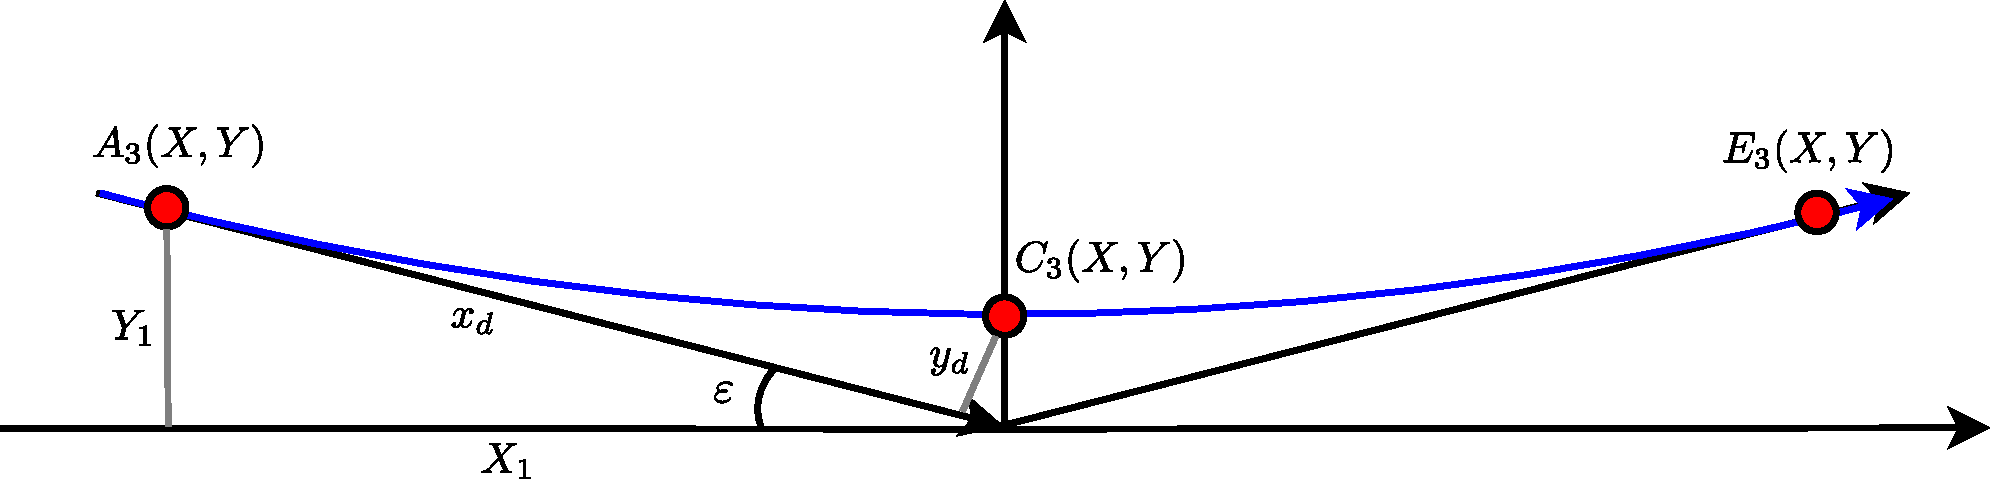
\includegraphics[width=8.4cm]{img/3Points} % width of a column is 8.4 cm.
		\caption{Path planning when $\varepsilon$ < $\varepsilon_{max}$, the path is composed by two identical but mirrored Euler-spirals. 3 key points are generated, denoted $A_3$, $C_3$ and $E_3$}
		\label{fig:3points}
	\end{center}
\end{figure}
The 3 key points are given by the coordinate sets:
\begin{align}
A_3 = (-X_1,Y_1),\, C_3 = (0,\frac{y_d}{cos(\varepsilon)}),\, E_3 = (X_1,Y_1)
\end{align}
From where the individual coordinates can be computed by simple trigonometric equations, if the angle of the turn $\varepsilon$ is known. $x_d$ and $y_d$ are the length of the scaled Euler-spiral, when the turn of the spiral equals to $\varepsilon$, where $x_d$ and $y_d$ represents the $(x,y)$ coordinate pair of the two normalized Fresnel integral functions with the same parameter $t$. 
\begin{align}
\varepsilon = \frac{\textrm{dx }F(t)}{\textrm{dy}} \quad \to \quad [x_d,y_d] = F^{-1}(\varepsilon)
\end{align}
Once the angle grows larger than $\varepsilon_{max}$ the system has to compute five key points, as the ship must transit onto a curve, and then back onto the Euler spiral ($\kappa_{Euler_{max}} = \kappa_{Arc}$) This adds the extra waypoints $B_5$ and $D_5$, the entry and exit points of the curve. The center of the circular path segment is $O_5$ and the radius is $R_{min} = \frac{1}{\kappa_{max}}$. The waypoints are depicted on figure (\ref{fig:5points}), thus augmenting the waypoints to:
\begin{figure}
	\begin{center}
		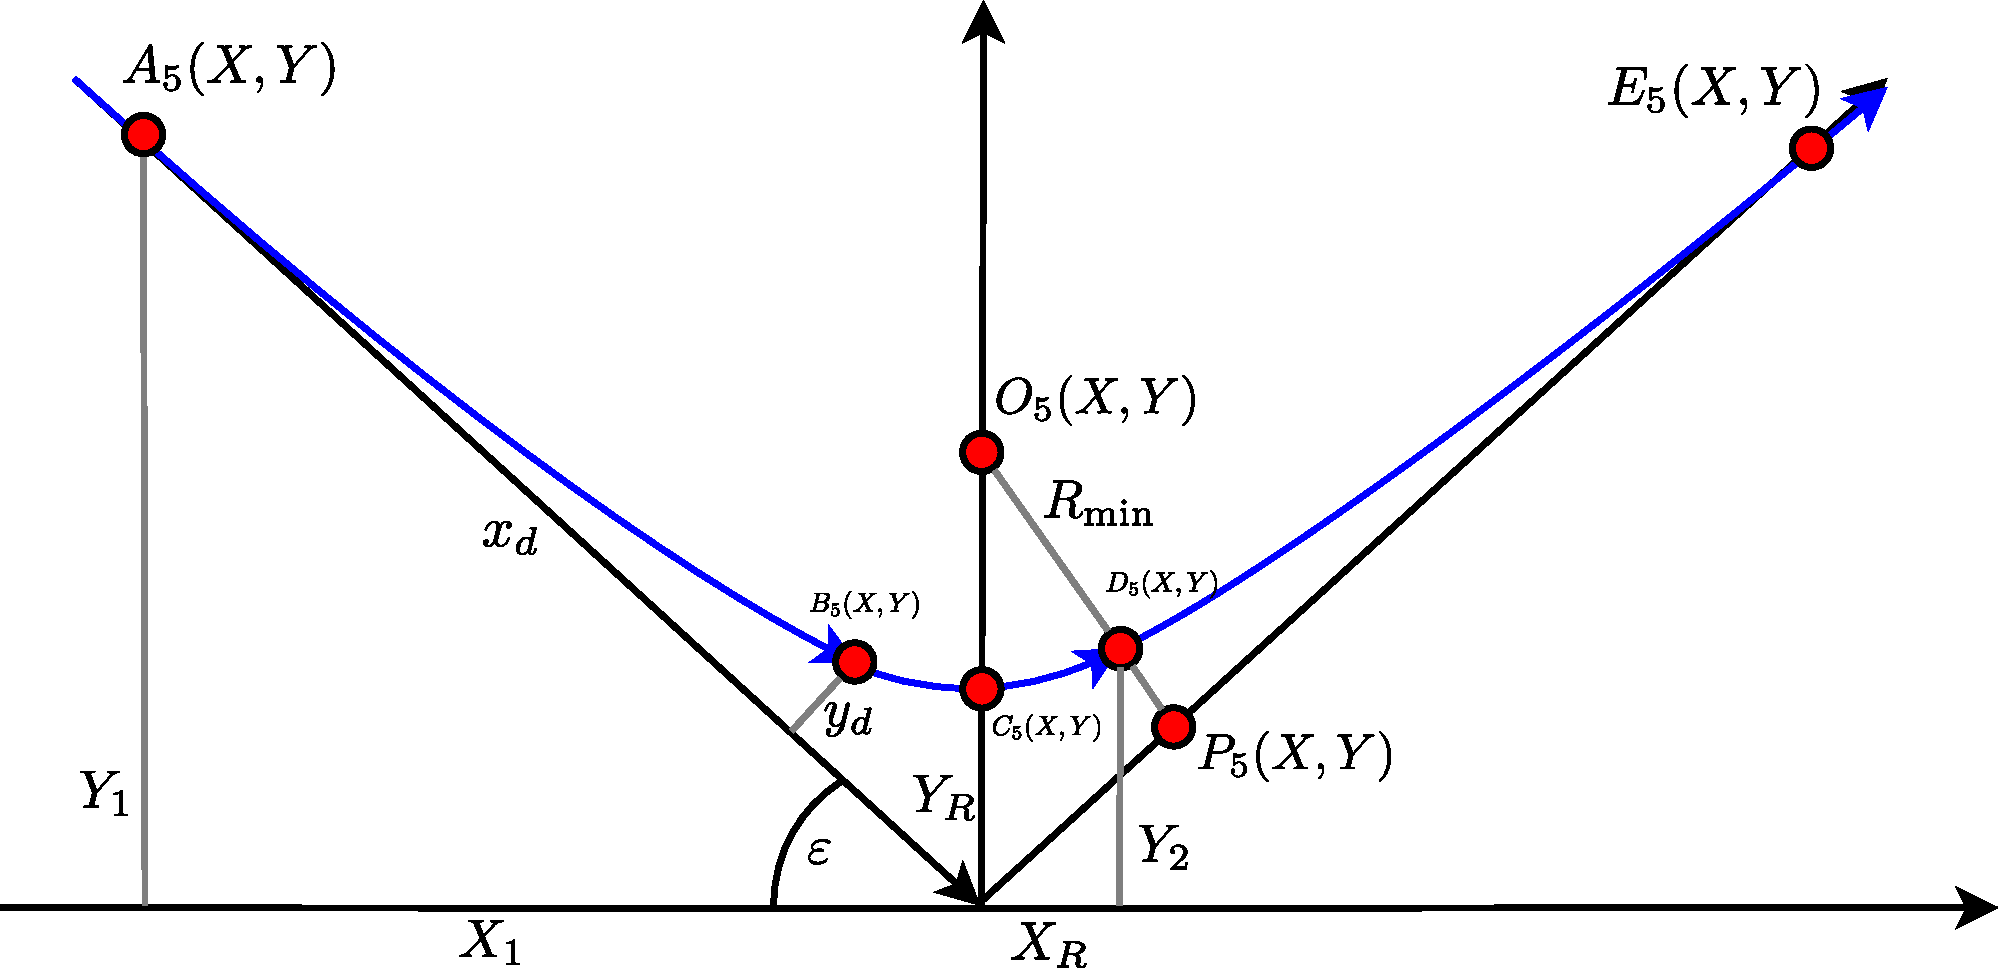
\includegraphics[width=8.4cm]{img/5Points}    % The printed column  
		\caption{Path planning when $\varepsilon$ < $\varepsilon_{max}$, the path is approximated by a curve and 5 key points are generated, denoted $A_5$, $B_5$, $C_5$, $D_5$ and $E_5$}  % width of a column is 8.4 cm.
		\label{fig:3points}               
	\end{center}                                 % accordingly.
\end{figure}
\begin{align}
A_5 &= (-X_1,Y_1),\, B_5 = (-X_2,Y_2),\, C_5 = (0,Y_R)\\
D_5 &= (X_2,Y_2),\, E_5 = (X_1,Y_1)
\end{align}
Which is still a mirroring of points about the $x=0$ axis, as the entry angle is the same as the exit angle. The number of equations increases, and the individual coordinates can be computed by:
\begin{align}
X_R &= R_\text{min} \cdot \sin(\varepsilon - \varepsilon _\text{max}),\,\, P_X = X_R + y_d \cdot \sin(\varepsilon)\\
X_1 &= P_X + x_d \cdot \cos(\varepsilon),\,\, Y_1 = X_1 \cdot \tan(\varepsilon)\\
P_Y &= Y_1 - x_d \cdot \sin(\varepsilon),\,\, Y_2 = P_Y + y_d \cdot \cos(\varepsilon)\\
O_Y &= R_\text{min} \cdot \cos(\varepsilon - \varepsilon _\text{max}) + Y_2,\,\, Y_R = O_Y - R_\text{min}\\
X_2 &= X_R
\end{align}

The resulting path in both cases can not be described explicitly, therefore a Hermite-polynom is fit to the key points. In addition, a predefined number of uniformly distributed sub-waypoints are generated on the path, based on the describing polynom. The resulting sub-waypoints are rotated and moved to their correct position in the Local-Frame, thus concluding most of the work of the local-planner. The paths between turns are straight lines, populated with the same preset density of sub-waypoints.

\subsection{Navigation}

The navigation controller of the ship is a general reference heading calculator, which outputs the required direction of movement to reach the next waypoint. In order to efficiently and accurately navigate along the path, a set of Sub-Waypoints is calculated for each route between two Waypoints. The main control strategy is to navigate through all of these SWPs in a predefined order, one by one. The heading of the ship is defined in NED\footnote[1]{[North, East, Down]} coordinate system. The required heading is determined based on the Position of the Ship and the Position of the next Sub-Waypoint.

\begin{figure}
	\begin{center}
		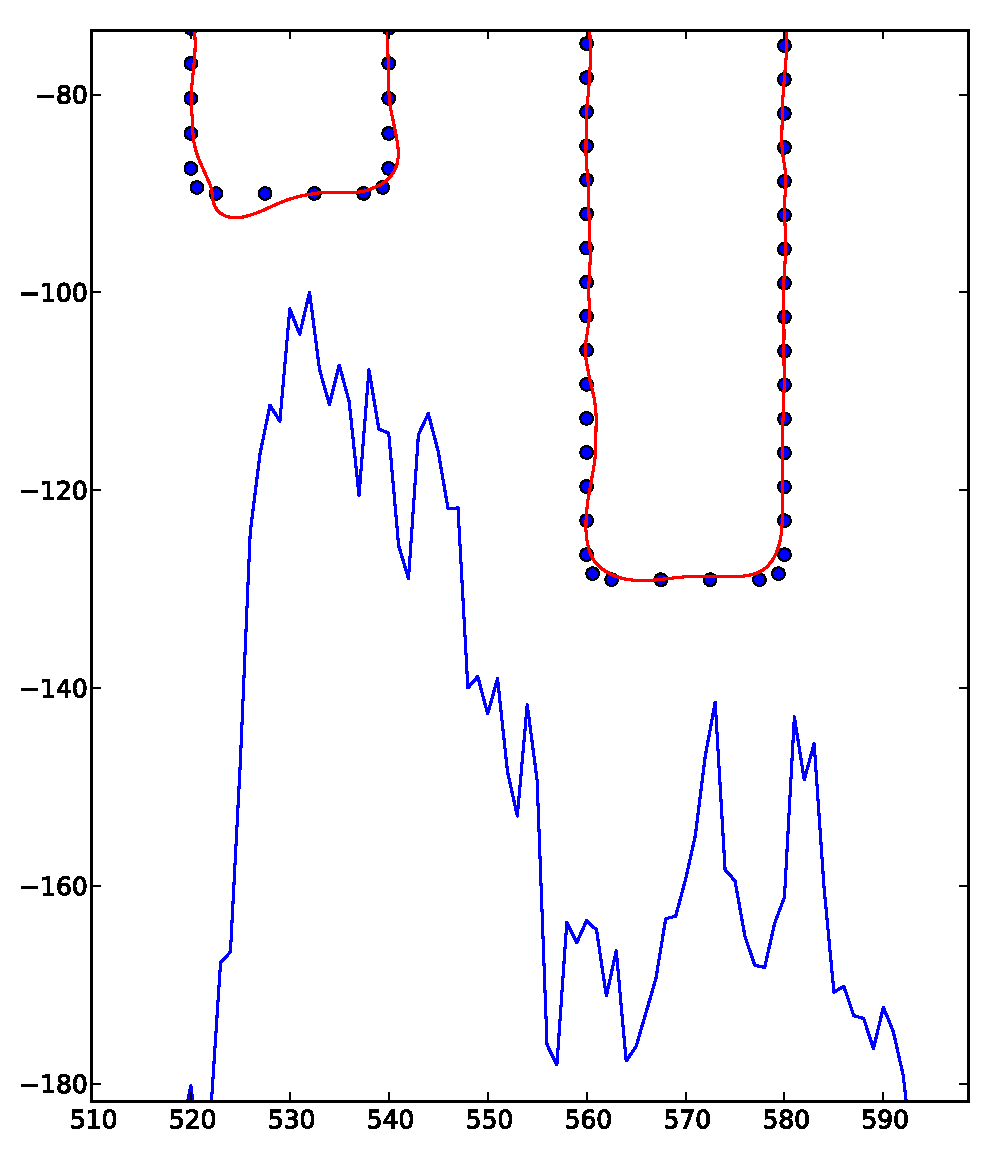
\includegraphics[width=8.4cm]{img/Navi}    % The printed column  
		\caption{Part of the simulated path of the embedded system close to the shore along the sub-waypoints, during a regular oceanography task, based on GPS position measurements affected by white noise with 4m variance}  % width of a column is 8.4 cm.
		\label{fig:navi}               
	\end{center}                                 % accordingly.
\end{figure}

\subsection{State estimation}
To give a better estimate of position and the attitude of the craft, a Kalman filter have been implemented to improve the accuracy of the sensors mounted aboard the ship. To develop a such, the discrete time state model of the ship have been derived to be:
\begin{align}
\vec{\Phi} = diag\{\vec{\Phi} _x,\vec{\Phi} _y,\vec{\Phi} _\omega\}
\end{align}
Where the diagonal entries $\vec{\Phi} _x,\vec{\Phi} _y,\vec{\Phi} _\omega$ are given by the same equation, with different entries:
\begin{align}
\vec{\Phi}_{x,y,\omega}(k) = \begin{bmatrix}
1 & t_s & 0\\
0 & 1 & t_s\\
0 & \frac{-\beta_{x,y,\omega}}{m,m,I} & 0
\end{bmatrix}
\end{align}
Where $\beta_{x,y,\omega}$ denotes the skin frictional drag in the $x$,$y$ or $\omega$ direction respectively, $m$ is the mass of the craft, $I$ is the inertia and $t_s$ is the sampling time of the filter. The states to be estimated for the controller are:
\begin{align}
^b\hat{\vec{x}_k} = \begin{bmatrix}
x & \dot{x} & y & \dot{y} & \theta & \omega
\end{bmatrix}^T
\end{align}
The observation model of the filter does however contain more measurements, and the measurements can be given as:
\begin{align}
\vec{v}_k = \begin{bmatrix}
x & \dot{x} & \ddot{x} & y & \dot{y} & \ddot{y} & \theta & \omega & \alpha
\end{bmatrix}^T
\end{align}
To tune the filter the covariance matrices $\vec{R}_k$ and $\vec{Q}_k$ are a function of the measurement distribution and the input distribution. The input to the system is given as:
\begin{align}
\vec{w}_k = \vec{B}\vec{u}
\end{align}
Where $\vec{B}$  is an augmented version of the system input matrix defined in INSERT REFERENCE! and $\vec{u}$ is the inputs to the system given as a force $F$ and a torque $\tau$. $\vec{B}$ is given as 
\begin{align}
\vec{B} = \begin{bmatrix}
0 & 0 & \frac{1}{m} & 0 & 0 & 0 & 0 & 0 & 0\\
0 & 0 & 0 & 0 & 0 & 0 & 0 & 0 & \frac{1}{I} \end{bmatrix}^T
\end{align} 
And the input is given as $\vec{u} = \begin{bmatrix}F\ & \tau\end{bmatrix}^T$. As $\vec{B}$ is a static matrix, it is only the distribution of the force $F$ and the torque $\tau$ that is of interest. The distribution of the force are split into an $x$-component and a $y$ component, as the ship is also expected to move in the $y$-direction. The distributions of the force is givne as white Guassian noise processes, thus stating:
\begin{align}
F&\sim \mathcal{N}(\vec{\mu}_F,\vec{\sigma}^2_F)\\
\tau&\sim \mathcal{N}(\mu_\tau,\sigma^2_\tau)
\end{align}
Where the tuning through simulations have yielded the best results using $\vec{\mu}_F = \begin{bmatrix}5.4355 & 0\end{bmatrix}^T$. The first entry is because to the ship is for most of the time moving along at 1 m/s and that is the estimated force required to thrust the ship forward at 1 m/s with the frictional drag the ship experiences. The latter is the force in the $y$-direction which is given as a zero-mean process as the ship is not expected to move sideways. The torque is also given as a zero-mean process as the ship for most of the time is moving straight. The covariance matrix for the input, can thus be given as the covariance of $\vec{B}\vec{u}$ which gives the following:
\begin{align}
\vec{R}_k = 
\end{align}

The implementation of the filter is an altered version of an Linear Minimum Mean Square Error filter - the alteration lies in the Kalman gain, where a matrix mask $\\vec{Lambda}$ is post multiplied. This matrix mask is to zero out the measurements that are invalid. This matrix mask is defined as:
\begin{align}
\vec{\Lambda} = diag\{\lambda_x,\lambda_{\dot{x}},\lambda_{\ddot{x}},\lambda_{\lambda{y}},\lambda_{\dot{y}},\lambda_{\ddot{y}},\lambda_{\theta},\lambda_{\omega},\lambda_{\alpha} \}
\end{align}
This ensures that when a measurement is invalid (the checksum is not true) the receiver zeros out the gain, and runs the filter on the other sensors / estimates. The individual $\lambda$s are thus given as:
\begin{align}
\lambda = 
\left\{
  \begin{array}{l l}
    1 & \quad \text{if checksum is valid}\\
    0 & \quad \text{otherwise}
  \end{array} \right.
\end{align} 
This makes sure to zero out the measurement if a packet is corrupted instead of making the filter run on faulty data. The below figure is a simulation run in MATLAB which plots the absolute error of the position estimates of the ship for three different cases, one where the Kalman filter is running ideally with all packages available, one where the system looses 5 percent of the packages and another where the ship looses 5 percent, but gains these packages with 0 in the Kalman gain. 
\begin{figure}
	\begin{center}
		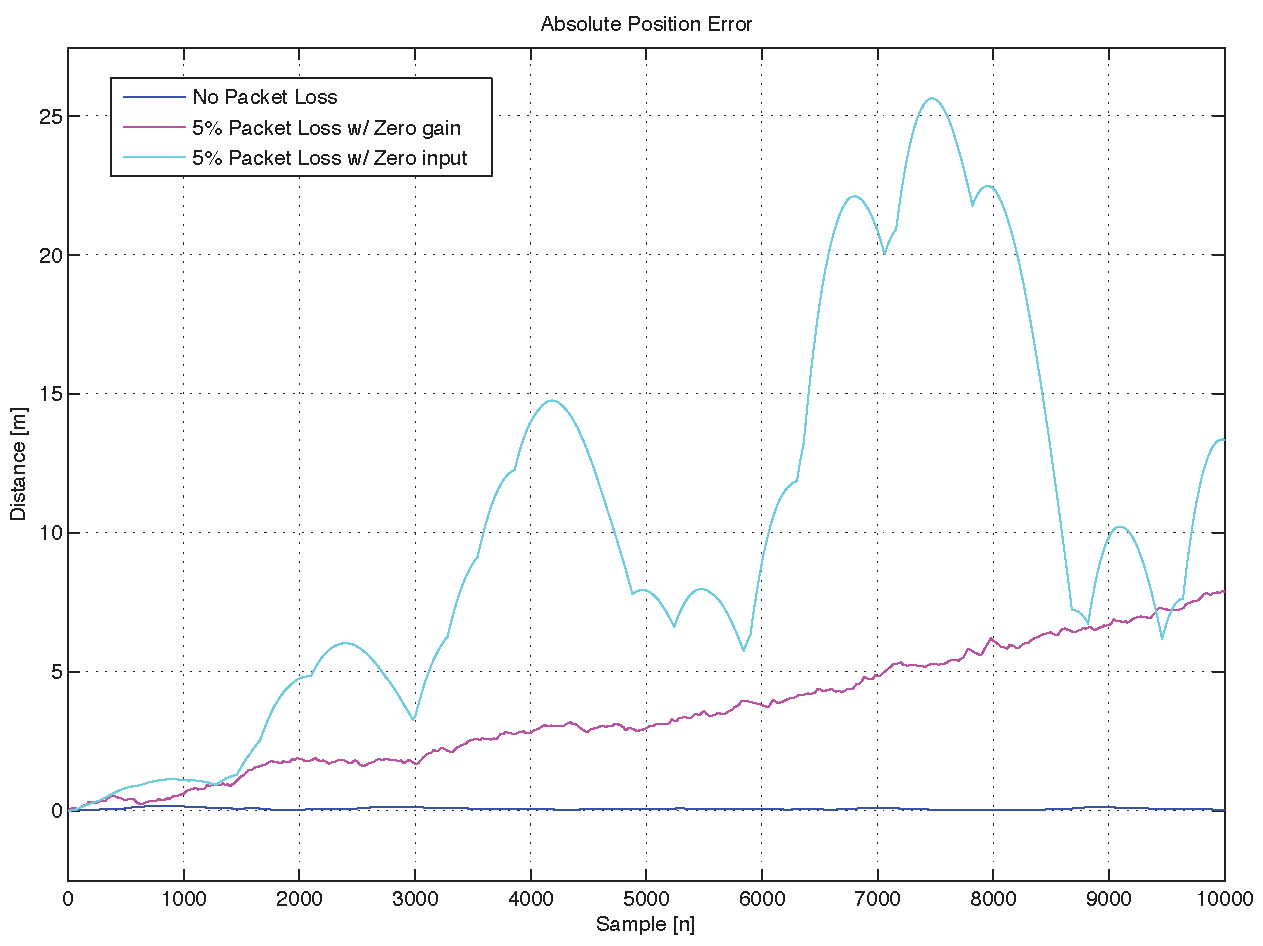
\includegraphics[width=8.4cm]{img/abspos}    % The printed column  
		\caption{Plot of the absolute position error, simulated using MATLAB and a sawtooth input to the control system running at }  % width of a column is 8.4 cm.
		\label{fig:3points}               
	\end{center}                                 % accordingly.
\end{figure}


As all the forces are acting on the ship in the inertial body fixed frame - the 

\section{Math}
Some mathematics go here. 

\section{Units}

\section{Results}

\subsection{Model of the ship}
The model of the ASV is in continuos time given as the state space equation defined in (eq:\ref{eq:ss_cont}) - the model considers the motion of the ship with 3 degrees of freedom, movement in the x-direction, y-direction and rotation about the z-axis. 
\begin{align}
\dot{\begin{bmatrix}
v\\
\theta\\
\omega
\end{bmatrix}} = \begin{bmatrix}
\frac{-\beta_v}{m} & 0 & 0\\
0 & 0 & 1\\
0 & 0 & \frac{-\beta_\omega}{I}
\end{bmatrix} + \begin{bmatrix}
\frac{1}{m} & 0\\
0 & 0\\
0 & \frac{1}{I}
\end{bmatrix}
\label{eq:ss_cont}
\end{align}
This model is sufficient as it is only the velocity and the angle that is desired to cont as the other states are uncontrollable by the ship in its current configuration. The control strategy is to track the input reference, and use an optimal feedback gain to reach the desired values. This is done as in REFERENCE! giving the following gains:
\begin{align}
F_opt &= \\
N &= 
\end{align}

A little about the way we get from a force input to an engine output:
As the controller outputs a force $F$ and a torque $\tau$ the controller must convert these to a set-point for the revolutions. The force of the forward motion of the ship is given as a function of the number of revolutions of the propeller $n$. The function is defined by \cite{cyber} as:
\begin{align}
F_1 &= C_1 \cdot |n_1| \cdot n_1\\
F_2 &= C_1 \cdot |n_2| \cdot n_2
\end{align}
Where $C_1 = \rho \cdot K_T \cdot D^4$, which are constants. The two propellers thus produce a total force as a function of their individual rotational velocities. The torque produced by the propellers can be described as the distance to the propeller and the angle out here. The angle is measured to be $\theta = \frac{pi}{16}$, thus giving the torque $\tau$ as a function of the starboard and port engines:
\begin{align}
\tau_1 &= F_1 \cdot \sin(\theta)\\
\tau_2 &= F_2 \cdot \sin(-\theta)\\
\end{align}
As the two engines both produce a force and a torque, given the same revolutions, the matrix equation $\vec{A}\vec{x} = \vec{b}$ can be solved to give:
\begin{align}
\begin{bmatrix}
n_1^2\\
n_2^2
\end{bmatrix} = \begin{bmatrix}
C_1 & C_1\\
C_1 \cdot \sin(\theta) & C_1 \cdot \sin(-\theta)
\end{bmatrix}^{-1}\begin{bmatrix}
F_\text{desired}\\
\tau_\text{desired}
\end{bmatrix}
\end{align}
Whats left to do is to solve for $n_1$ and $n_2$. These can be solved by:
\begin{align}
n_1 = \frac{n_1^2}{\text{abs}\{n_1^2\}} \cdot \sqrt{\text{abs}\{n_1\}}\\
n_2 = 
\end{align}


\subsection{Control verification}
Running the system with just the controllers produces the following plot trying to follow a path around the parking lot. 

\subsection{Path planning results}
Planning the path on a stretch of water in Aalborg produces the following results:

\subsection{Kalman filtering verification}
Filtering the above traced controller route with the Kalman filter, having the input to the system to zero, and post processing the data produces the following plot.

\subsection{Combined test}
Running the Kalman filter on the ship whilst in motion. As seen some packages are lost - to verify the simulator, a simulation have been run with the same amount of packages lost, and this produces the same result. 

Something about the packet loss. 

\subsection{Other tests}

Something else?


\section{Conclusion}

A conclusion section is not required. Although a conclusion may review the main points of the paper, do not replicate the abstract as the conclusion. A conclusion might elaborate on the importance of the work or suggest applications and extensions. 

\begin{ack}                               % Place acknowledgements
A special thank should be given to Assistant Professor Carles Navarro Manchòn, Section for Navigation and Communication, Department of Electronic Systems, Aalborg University for his help with tuning the Kalman filter.  % here.
\end{ack}

%\bibliographystyle{alpha}        % Include this if you use bibtex 
%\bibliography{autosam}           % and a bib file to produce the 
%\bibliography{autosam}
                                 % bibliography (preferred). The
                                 % correct style is generated by
                                 % Elsevier at the time of printing.

\begin{thebibliography}{xx}

\bibitem[Talbot (1901)]{Art:1}
Arthur N. Talbot,
\newblock \emph{The Railway Transition Spiral}
\newblock The Engeneering News Publishing Co., 1901

\bibitem[K\'oml\'osi-Kiss (2011)]{Art:2} % The name shown in the report, and the lable \cite{Art:1}
Istv\'a n Koml\'{o}si \& B\'a lint Kiss, % Name of the author
\newblock \emph{Mobilis robotok auton\'{o}m navig\'aci\'{o}ja mozg\'{o} akad\'alyok elker\"ul\'es\'evel} % The name of the thesis
\newblock Budapest University of Technology and Economics, 2011 % The publisher

\bibitem[S\o rensen (2005)]{cyber}
Asgeir J. S\o rensen,
\newblock \emph{Marine Cybernetics, Modelling and Control - Lecture Notes}
\newblock Department of Marine Cybernetics, Norwegian University of Science and Technology, 2005

\end{thebibliography}








\appendix
\section{A summary of Latin grammar}    % Each appendix must have a short title.
\section{Some Latin vocabulary}         % Sections and subsections are supported  
                                        % in the appendices.
\end{document}
